\documentclass[12pt,crop,tikz,convert={outext=.svg,command=\unexpanded{pdf2svg\space\infile\space\outfile}}]{standalone}
\usepackage[utf8]{inputenc}
\usepackage[T1]{fontenc}
\usepackage{tikz}

\begin{document}
  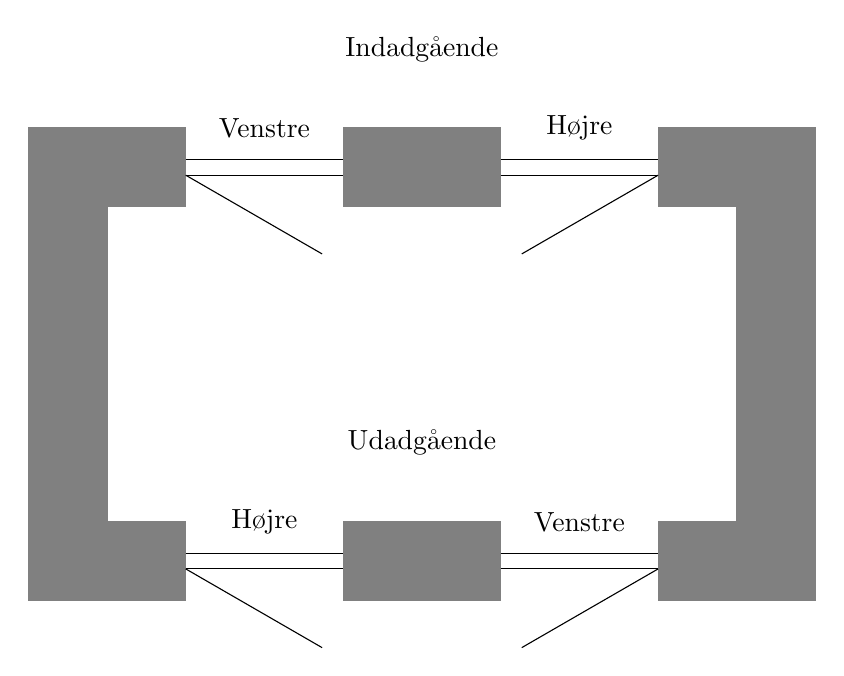
\begin{tikzpicture}
    \begin{scope}
      \foreach \i in {-1,3,7}
        \filldraw[gray] (\i,0) rectangle (\i+2,1);
      \foreach \i in {1,5}
	\draw (\i,0.4) -- (\i+2,0.4);
      \foreach \i in {1,5}
	\draw (\i,0.6) -- (\i+2,0.6);
      \draw[rotate around={-30:(1,0.4)}] (1,0.4) -- (3,0.4);
      \draw[rotate around={30:(7,0.4)}] (7,0.4) -- (5,0.4);
      \draw (4,2) node {Indadgående} (2,1) node {Venstre} (6,1) node {Højre};
    \end{scope}

    \begin{scope}[yshift=-5cm]
      \foreach \i in {-1,3,7}
        \filldraw[gray] (\i,0) rectangle (\i+2,1);
      \foreach \i in {1,5}
	\draw (\i,0.4) -- (\i+2,0.4);
      \foreach \i in {1,5}
	\draw (\i,0.6) -- (\i+2,0.6);
      \draw[rotate around={-30:(1,0.4)}] (1,0.4) -- (3,0.4);
      \draw[rotate around={30:(7,0.4)}] (7,0.4) -- (5,0.4);
      \draw (4,2) node {Udadgående} (6,1) node {Venstre} (2,1) node {Højre};
    \end{scope}

    \foreach \i in {-1,8}
      \filldraw[gray] (\i,1) rectangle (\i+1,-4);

  \end{tikzpicture}
\end{document}
